\chapter{Mechanical testing of cured laminates}
\label{mechanical}

\section{Interlaminar Shear Strength}
\label{sec:ilss}

Interlaminar shear test shall be done according EN 2563 for ATL material and ASTM D2344 for AFP material. As so, specimen dimensions should be as follow for both ATL and AFP material, in table \ref{table:dimensionsils}. \gls{ils} is one of the most useful tests while testing laminates, since is relatively easy to execute, is quick, cheap (due to reduced specimen dimensions) and is representative of the process. Specimens are to be cut through CNC waterjet machine.

% Please add the following required packages to your document preamble:
% \usepackage{booktabs}
\begin{table}[htbp]
\centering
\caption{Specimen dimensions for \gls{ils} test}
\label{table:dimensionsils}
\setlength\aboverulesep{0pt}\setlength\belowrulesep{0pt}
	\begin{tabular}{@{}c|cc@{}}
		Material & Dimension (mm)                     & Thickness (nr. of plies) \\ \midrule
		ATL      & 20,0 $\pm$ 0,25 x 10,0 $\pm$ 0,2   & 11                       \\
		AFP      & ($6*t \pm$ 0,25) x ($2*t \pm$ 0,2) & 12                      
	\end{tabular}
\end{table}

\subsection{Specimen preparation}
\label{ilss:specimenprep}

\subsection{Test and machine preparation}
\label{ilss:testprep}

\subsection{Results and discussion}
\label{ilss:results}

\section{Interlaminar Tension Strength}
\label{sec:ilts}

Interlaminar Tension Strength shall be done according to ASTM D6415, in which the specimens are stated for both ATL and AFP material, in figure \ref{fig:dimensionsilts}. These specimens are going to be manufactured in a 'L' shaped mold, in order to provide the necessary angle and shape to the specimens for testing. Due to exposure condition number 1 (section \ref{expcond}), some hand lay-up was needed and developed using this method (more on detail in annex):

\begin{enumerate}
	\item Using ATL or AFP, lay-up up to 6 plies in a flat surface;
	\item Hand lay-up the 6-ply laminate into the mold surface and apply vacuum;
	\item Repeat until all plies are laminated.
\end{enumerate}

\texorpdfstring{\gls{ilts}} specimens shall be cut by disk cutter thanks to the imposed 90º angle that makes it a near impossible task to cut by CNC waterjet machine. However, a test was conducted to assess disk cutter ability to cut specimen without damaging edges and generate delaminations. The arrangement was that specimens would be cut with disk cut aided with water as lubricant, with the nuance that an excess would be added, providing room to sanding the excess and assure specimen quality.

\begin{figure}[htbp]
\centering
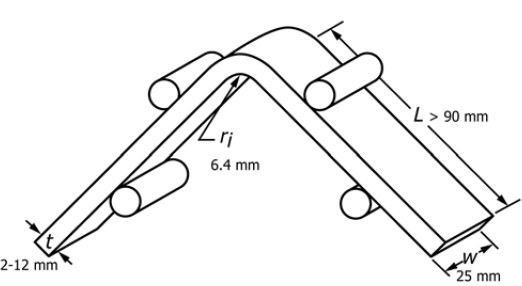
\includegraphics[scale=0.6]{Chapters/Figures/ilts}
\caption{Dimensions for ILTS specimens \cite{ASTMInternational2013}}
\label{fig:dimensionsilts}
\end{figure}

\subsection{Specimen preparation}
\label{ilts:specimenprep}

\subsection{Test and machine preparation}
\label{ilts:testprep}

\subsection{Results and discussion}
\label{ilts:results}